%! TEX program = luatex
%% ****** Start of file aiptemplate.tex ****** %
%%
%%   This file is part of the files in the distribution of AIP substyles for REVTeX4.
%%   Version 4.1 of 9 October 2009.
%%
%
% This is a template for producing documents for use with 
% the REVTEX 4.1 document class and the AIP substyles.
% 
% Copy this file to another name and then work on that file.
% That way, you always have this original template file to use.
% chktex-file 36
\documentclass[aps,prl,preprint,superscriptaddress]{revtex4-1} % chktex 8
%\documentclass[aip,reprint]{revtex4-1}
\usepackage{amsmath}
\usepackage{graphicx}
\usepackage{siunitx}
%\usepackage[english]{babel}
%\usepackage{upgreek}
%\usepackage[math-style=ISO]{unicode-math}
%\usepackage[upright]{fourier}
%\usepackage{newtxmath}
\usepackage{xcolor}
\bibliographystyle{unsrt}
\raggedbottom%
\def\nm{\,\si{\nano\meter}}% 
\draft% marks overfull lines with a black rule on the right
\begin{document}

% Use the \preprint command to place your local institutional report number 
% on the title page in preprint mode.
% Multiple \preprint commands are allowed.
%\preprint{}

\title{Shape Matters in Magnetic-field Assisted Assembly of Colloidal Ellipsoids}

% repeat the \author .. \affiliation  etc. as needed
% \email, \thanks, \homepage, \altaffiliation all apply to the current author.
% Explanatory text should go in the []'s, 
% actual e-mail address or url should go in the {}'s for \email and \homepage.
% Please use the appropriate macro for the type of information

% \affiliation command applies to all authors since the last \affiliation command. 
% The \affiliation command should follow the other information.

%\author{}

\author{Antara Pal}
\email{antara.pal@fkem1.lu.se}
\affiliation{Division of Physical Chemistry, Department of Chemistry, Lund University, Lund, Sweden}
\author{Carlo Andrea De Filippo}
\affiliation{Science Department, University Roma Tre, Via della Vasca Navale 84, Roma, Italy}
\author{Thiago H.Ito}
\affiliation{Division of Physical Chemistry, Department of Chemistry, Lund University, Lund, Sweden}
\author{Md. Arif Kamal}
\affiliation{Centre Interdisciplinaire de Nanoscience de Marseille (CINaM), CNRS, Aix Marseille University, Marseille, France}
\altaffiliation[Current Address: ]{Division of Physical Chemistry, Department of Chemistry, Lund University, Lund, Sweden}
\author{Andrei V. Petukhov}
\affiliation{Van't Hoff Laboratory for Physical and Colloid Chemistry, Utrecht University, The Netherlands}
\author{Cristiano De Michele}
\affiliation{Department of Physics, Universit\`{a} di Roma La Sapienza, I-00186 Roma, Italy}
\author{Peter Schurtenberger}
\email{peter.schurtenberger@fkem1.lu.se}
\affiliation{Division of Physical Chemistry, Department of Chemistry, Lund University, Lund, Sweden}

% Collaboration name, if desired (requires use of superscriptaddress option in \documentclass). 
% \noaffiliation is required (may also be used with the \author command).
%\collaboration{}
%\noaffiliation

\date{\today}

\begin{abstract}
%-----------------------------------------------------
Anisotropic colloids exhibit a rather complex and rich phase behavior in comparison to their isotropic analogues, which renders them as interesting model systems in various areas of condensed matter physics and materials science. Herein we present our investigation of the influence of an external magnetic field on the self-assembly of hematite-silica core-shell ellipsoidal colloids. In the presence of an external field, prolate particles usually orient with their long axes along the field direction. However, our study has brought to light a rather counterintuitive but interesting phenomenon where \emph{prolate} anisotropic colloids self-assemble into \emph{oblate} liquid crystalline (LC) phases. This \emph{unusual} self-assembly behaviour can be attributed to an inherent peculiarity in the magnetic property of hematite, due to which, the particles align with their short axes along the field direction. Detailed characterization of the concentration dependent self-assembly process using particles with two different but relatively small aspect ratios (AR) reveal that self-assembly is sensitive to the particle AR\@. For particles with the smaller AR, an increase in concentration results in the formation of a sequence of oblate LC phases: \emph{para-nematic}, \emph{nematic}, \emph{smectic} and an \emph{oriented glass}. Remarkably, the occurrence of a smectic phase in colloidal ellipsoidal systems has neither been predicted by simulations nor previously reported experimentally. \textcolor{red}{A quantitative image analysis of the two types of particles and a comparison with extensive computer simulations where we investigate self-assembly of particles with different prolate shapes in the presence of a magnetic field indicates that it is not only the aspect ratio but subtle shape changes that are responsible for the highly unusual sequence of field-induced structures observed for the smaller aspect ratio particles. }Our study unequivocally demonstrates the power of combining anisotropic building blocks and external fields as a route towards field-directed self-assembly of novel structures with externally tunable properties. 
%-----------------------------------------------------
\end{abstract}

\pacs{}% insert suggested PACS numbers in braces on next line

\maketitle {}%\maketitle must follow title, authors, abstract and \pacs

% Body of paper goes here. Use proper sectioning commands. 
% References should be done using the \cite, \ref, and \label commands
\section{Introduction}
%\label{}
%-----------------------------------------------------------------------------------------------------------------------------------
Over the past couple of decades the focus of colloid science has gradually witnessed a shift towards understanding the behavior of anisotropic particles; particles having anisotropy either in their shape or interaction potential or both. Anisotropic colloids exhibit a rather complex and rich phase behavior in comparison to their isotropic analogues, which makes them particularly interesting model systems in various areas of condensed matter physics and materials science. The prospect of tuning their self-organization by modifying the anisotropy in their shape in conjunction with the possibility of introducing an anisotropy in the interaction potential using external fields have ushered in a new paradigm towards the understanding, design and control of novel self-assembled materials. \par
%-----------------------------------------------------------------------------------------------------------------------------------
Depending upon the particle shape and the interaction potential, suspensions of aniso\-tropic colloids manifest different
self-assembled structures encompassing \emph{isotropic}, 
\emph{nematic}~\cite{pizzey2004suspensions, van1998formation, purdy2005nematic, buining1993isotropic, fraden1989isotropic, lemaire2002outstanding, lemaire2004physical, vroege2014biaxial, van2010uniaxial, rossi2010cholesteric, li2016colloidal,dogic2016filamentous}, 
\emph{smectic}~\cite{davidson2018isotropic, vroege2006smectic, kuijk2012phase} and \emph{columnar} phases~\cite{van2000liquid, brown1999phase, wijnhoven2005sedimentation, van2004liquid, van2005evidence}. 
One of the most important feature that distinguishes these phases from one another is the presence (or absence) of orientational and positional order. In the isotropic phase the particles possess neither 
orientational nor positional order, whereas in the nematic phase there exists a long-range orientational order but an absence of long-range positional order. 
Smectic and crystal phases are generally characterized by the presence of both long-range orientational as well as positional order. \par
%-----------------------------------------------------------------------------------------------------------------------------------
The use of external electromagnetic fields to manipulate the orientational interactions of anisotropic particles and drive their self-assembly has been in the spotlight for the last couple of years (ref.~\cite{op2013phase, Schurtenberger2016, ganesan2017high, shah2015actuation} and references therein). The fast and reversible nature of the field-induced dipole-dipole interaction between the particles, as is the case in these systems, makes this bottom-up approach extremely versatile. In view of the ease in manipulating the interaction potential of magnetic particles through external field, we have in the present study focused our attention towards investigating field-directed self-assembly of ellipsoidal particles with a magnetic core.\par
%-----------------------------------------------------------------------------------------------------------------------------------
Over the past decade a significant amount of work has been done towards elucidating the theoretical phase diagrams for ellipsoidal particles. These studies predict the existence of isotropic, nematic and SM2 crystalline phases as a function of concentration and axial ratio~\cite{radu2009solid, odriozola2012revisiting, pfleiderer2008crystal}. It is interesting to note that so far there are neither any predictions nor any experimental reports for the existence of a smectic phase in case of ellipsoidal particles. This is in stark contrast to the situation encountered for example for particles with cylindrical or spherocylindrical shapes~\cite{Bolhuis1997, lekkerkerker2013liquid}. In this article we have not only revisited these theoretical predictions for ellipsoidal particles, but have in addition used an external field to investigate the effect of a partial reduction in the rotational degrees of freedom of the ellipsoids.\par
%%%----------------------------------------------------------------------------------------------
In the case of anisotropic particles, the presence of an external magnetic field results in an alignment of the magnetic moment of the individual particles along the field direction, thereby restricting rotational motion of the particles accordingly. For prolate particles the induced dipolar moments are in general along their long axis. However, this is not the case for prolate particles consisting of a magnetic core that is made up of hematite ($\alpha$-Fe$_2$O$_3$) spindles. In this scenario, the particles align with their short axis parallel to the field direction~\cite{reufer2011magnetization,reufer2010morphology}. The explanation of this rather striking behaviour rests on the fact that in case of hematite the easy axis of magnetization resides within the basal plane of the hematite and is oriented perpendicular to the spindle axis. Consequently, the direction of the induced magnetic moments is perpendicular to the long axes. Although at sufficiently large field strengths the particles align with their short axis parallel to the magnetic field, they can however still individually rotate around their magnetic moments provided the volume fraction is low enough and interparticle interactions are negligible~\cite{reufer2010morphology}. \par
%---------------------------------------------------------------------
In the present article, we have exploited the aforementioned property of hematite to tune the self-assembly of colloidal ellipsoids for two different aspect ratios of $\rho = 2.82$ and $\rho = 3.69$ at different concentrations. Using gravity to create a sedimentation profile (or concentration gradient) in a dispersion of silica coated hematite ellipsoids allows us to efficiently sample a large range of the phase space within a single sample. We report that for the ellipsoidal particles with the smaller aspect ratio ($\rho=2.82$) four different self-assembled structures exist: \emph{para-nematic}, \emph{nematic}, \emph{smectic} and \emph{oriented glass}, respectively. A quantitative analysis of the SAXS patterns clearly reveals that it is possible to create oblate self-assembled phases with prolate particles through the application of an external field. Astonishingly, our data unambiguously demonstrates the existence of a smectic phase in a colloidal ellipsoidal system, which has been neither predicted by simulations nor previously found experimentally. In the smectic phase, the SAXS pattern exhibits a curious peak shape that resembles a \textit{paper-clip} with highly anisotropic tails along the direction of the smectic periodicity. The presence of this unusual peak structure is rationalized by the modulation of the intensity in the form of a spherocylinder due to the correlation between the particles along different directions together with a layer undulation. \textcolor{red}{In contrast, ellipsoids with a higher aspect ratio of $\rho=3.69$ were found to self-assemble in only two different phases --- \emph{para-nematic} and \emph{nematic}. While the theoretical phase diagrams for ellipsoids without external fields show the same sequence of phases and only small quantitative differences in the location of the corresponding phase boundaries within this range of axial ratios, this seems to change dramatically with the existence of an external field. In order to understand the origin of these observations, we have therefore combined our SAXS experiments with computer simulations, where we use different geometrical models to investigate the effects of an external field and an increasing concentration on the phase behavior of these systems. In addition, we have also performed a detailed quantitative shape analysis of our two model systems using transmission electron microscopy. Our study indicates that small but systematic deviations of the actual particle shape from the ideal ellipsoidal shape combined with the unusual magnetic properties of hematite are at the origin of this hitherto not observed possibility to create an (oblate) smectic phase with prolate particles, demonstrating the importance of subtle effects of shape anisotropy in field-directed self-assembly. }
%---------------------------------------------------------------------
\begin{figure}[!h]
\centering{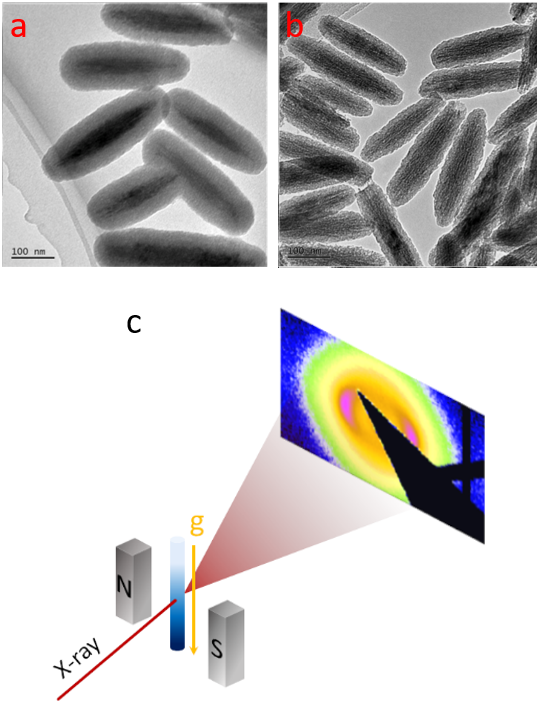
\includegraphics[width=0.5\linewidth]{TEM_2.png}}
\caption{TEM images for ellipsoidal colloids for aspect ratios (a) $\rho_1=2.82$ and (b) $\rho_2=3.69$. (c) Experimental set-up for SAXS measurement.}\label{TEM}
\end{figure}
%----------------------------------------------------------------------------------------------------------------
\section{Results and discussion}
%----------------------------------------------------------------------------------------------------------------
\subsection{Sample $E1$ with aspect ratio $\rho_1 = 2.82$}
%----------------------------------------------------------------------------------------------------------------
\begin{figure*}[t]
\centering{\includegraphics[width=0.95\textwidth]{Figure_Zscan_06.png}}
\caption{Typical 2D diffraction patterns for (a) para-nematic, (b) nematic, (c) smectic and (d) oriented glass phases at different heights of the sedimented sample for $\rho=2.82$. The variation of the scattered intensity as a function of scattering vector, $q$, for the aforementioned self-assembled phases along the direction of the external field (e) and perpendicular to it (f). (g) The variation of the nearest neighbor distance, $d$, and the FWHM of the nearest neighbor peaks as a function of height, $Z$ from the bottom of the capillary have been represented by the blue circles and the red squares respectively. The bottom panel represents schematic of the aforementioned self-assembled phases.}\label{z_scan}
\end{figure*} 
%----------------------------------------------------------------------------------------------------------------
The ellipsoidal system studied here exhibits a rich phase behavior involving para-nematic (pN)\footnote{The pN phase has been described before as a polarized fluid in ref.~\cite{martchenko2016anisotropic}}, nematic (N), smectic (S) and oriented glass (OG) phases \textcolor{red}{or states}. At the top of the sedimentation profile the concentration is relatively low, resulting in weak inter-particle correlations. As a result, the field-induced torque is mostly exerted onto single particles, resulting in an alignment that leads to the formation of a para-nematic phase (Fig.\ref{z_scan}(a)). A nematic phase followed by a smectic one is observed as one moves lower down in the capillary (Fig.~\ref{z_scan}(b), (c)). At the bottom of the sediment, due to the very high concentration, the particles form a kinetically arrested glass phase. In the presence of an external field, the particles tend to align with their short axes parallel to the field direction. As a result, the glass phase develops an anisotropy (Fig.\ref{z_scan}(d)). The nematic phase found for colloidal rods, which align their long axis, is often referred to as a \emph{prolate nematic}, N$_+$, while plate-like colloids exhibit an \emph{oblate nematic}, N$_-$, where the short particle axes are aligned. It is interesting to note that despite the prolate shape of our ellipsoidal particles their orientational behaviour in the presence of the external field closely follows that of oblate particles. This behaviour can be rationalized when one considers the fact that the ellipsoids consist of a hematite core. As a result, their magnetic moments lie along the short axes of the particles. Under the influence of an external magnetic field these particles self assemble with their short axes parallel to the field direction, thereby resembling oblate particles rather than rods. One can therefore refer to the field induced nematic, smectic and para-nematic phases as N$_-$, S$_-$ and pN$_-$ respectively, which is in strong contrast to the phases observed for colloidal rods~\cite{kuijk2011synthesis}. \par
%----------------------------------------------------------------------------------------------------------------
Fig.\ref{z_scan}(e) and (f) represent one-dimensional intensity profiles for different phases along and perpendicular to the direction of the field, respectively. At the very top of the sediment, in the pN phase, one can observe only the form factor, which is highly anisotropic; extending to larger $q$ along the field direction and decaying much faster in a direction perpendicular to the field direction (Fig.\ref{z_scan}(e)(f)(red)). This indicates that the particles are aligned with their short axes parallel to the field direction. At sufficiently high concentrations, positional correlations start to play an important role for the scattering in the direction parallel to the magnetic field. As a result, the static structure factor dominates the intensity profile, and we observe the appearance of additional well-developed maxima. The presence of very sharp smectic reflections up to fourth order along the direction of the field indicates a highly ordered structure (Fig.\ref{z_scan}(e)(cyan)). These strong positional and orientational correlations disappear again at the highest concentrations in the OG phase, where only a clear structure factor peak related to side-by-side correlations of the particles is observed parallel to the field direction(Fig.\ref{z_scan}(e)(blue)). In contrast, the scattering features are much less clearly developed in a direction normal to the field direction, and we only observe weak correlation peaks originating from the tip-to-tip configurations, i.e., with a separation distance equal to the particle length, for the nematic, smectic and oriented glass phases (Fig.\ref{z_scan}(f)). \par
%----------------------------------------------------------------------------------------------------------------
\textcolor{red}{In a vertical scan, the nearest neighbor distance $d$ $(=2\pi/q_{max})$ along the direction of the field increases as a function of the sample height $Z$ (Fig.\ref{z_scan}(g)), reflecting the decrease in concentration with increasing $Z$.} The full-width at half-maximum (FWHM) of the diffraction peak, which represents the inverse of the positional correlations, also changes as a function of $Z$ (Fig.\ref{z_scan}(g)). For the oriented glass and the nematic phase, the FWHM is quite large, indicating the presence of liquid-like positional order. In case of the smectic phase, however, there is a sharp decrease in FWHM, demonstrating the existence of a one-dimensional crystalline order.\par   % chktex 35
%----------------------------------------------------------------------------------------------------------------
\subsubsection{Characterization of the Nematic Phase}
%----------------------------------------------------------------------------------------------------------------
\begin{figure}[ht]
\centering{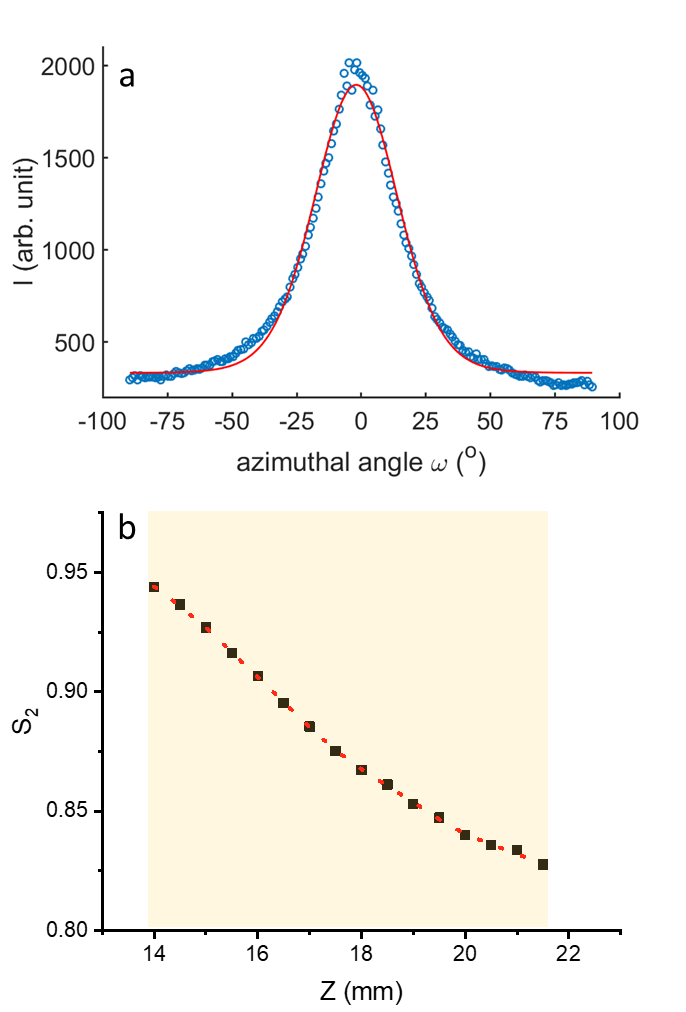
\includegraphics[width=0.5\linewidth]{order_param_5.png}}
\caption{(a) The blue circles represent the azimuthal intensity profile along the red dashed line shown in Fig.\ref{z_scan}(b) and the corresponding fit using eq.\ref{eq2:}(red line). (b) The variation of the orientational order parameter $S_2$ as a function of $Z$ in the nematic phase. The red dashed line is a guide to the eye but not a fit.}\label{order_param}
\end{figure} 
%----------------------------------------------------------------------------------------------------------------
The nematic phase is characterized by short-range positional order but long-range orientational order, which can be represented with the help of an orientational order parameter, $S_2$. Following Purdy \emph{et.~al.}~\cite{purdy2003measuring, kleshchanok2010structures}, the azimuthal intensity distribution (along the red dashed line in Fig.~\ref{z_scan}(b)) can be fitted with,
%----------------------------------------------------------------------------------------------------------------
\begin{equation}
\label{eq2:}
%\begin{split}
I= baseline +  I_0 f(\omega)
%\end{split}
\end{equation} 
%----------------------------------------------------------------------------------------------------------------
\noindent where $I_0$ is the normalizing factor, $\omega$ is the azimuthal angle and $f(\omega)$ is the orientational distribution function,
%----------------------------------------------------------------------------------------------------------------
\begin{equation}
\label{eq3:}
%\begin{split}
f(\omega)=\exp(-AP(\omega))
%\end{split}
\end{equation} 
%----------------------------------------------------------------------------------------------------------------
%\noindent where $A$ is the width of the Legendre polynomial,
\noindent where the parameter $A$ determines the width of the distribution function and $P(\omega)$ is the Legendre polynomial
%----------------------------------------------------------------------------------------------------------------
\begin{equation}
\label{eq4:}
%\begin{split}
P(\omega)=\frac{1}{2}(3\cos^2(\omega-\omega_0)-1)
%\end{split}
\end{equation} 
%----------------------------------------------------------------------------------------------------------------
\noindent with $\omega_0$ being the tilt angle. The orientational order parameter, $S_2$, can now be obtained by,
%----------------------------------------------------------------------------------------------------------------
\begin{equation}
\label{eq5:}
%\begin{split}
S_2= \frac{\int f(\omega)P(\omega)\sin(\omega)d\omega}{\int f(\omega)\sin(\omega)d\omega}
%\end{split}
\end{equation}
%----------------------------------------------------------------------------------------------------------------
\noindent Fig.\ref{order_param}(a) shows a representative fit of the experimental data with the Purdy model, while Fig.\ref{order_param}(b) represents the variation of $S_2$ as a function of $Z$. The analysis reveals that one of the short axes of the ellipsoids are very well aligned throughout the nematic phase, resulting in an order parameter $>$ 0.8. An interesting observation is that the order parameter is larger at the bottom part, indicating that the sample is more ordered, which is expected due to the sedimentation-induced concentration gradient.\par
%------------------------------------------------------------------------------------------------------------------
\subsubsection{Characterization of the Smectic Phase}
%------------------------------------------------------------------------------------------------------------------
\begin{figure}[ht]
\centering{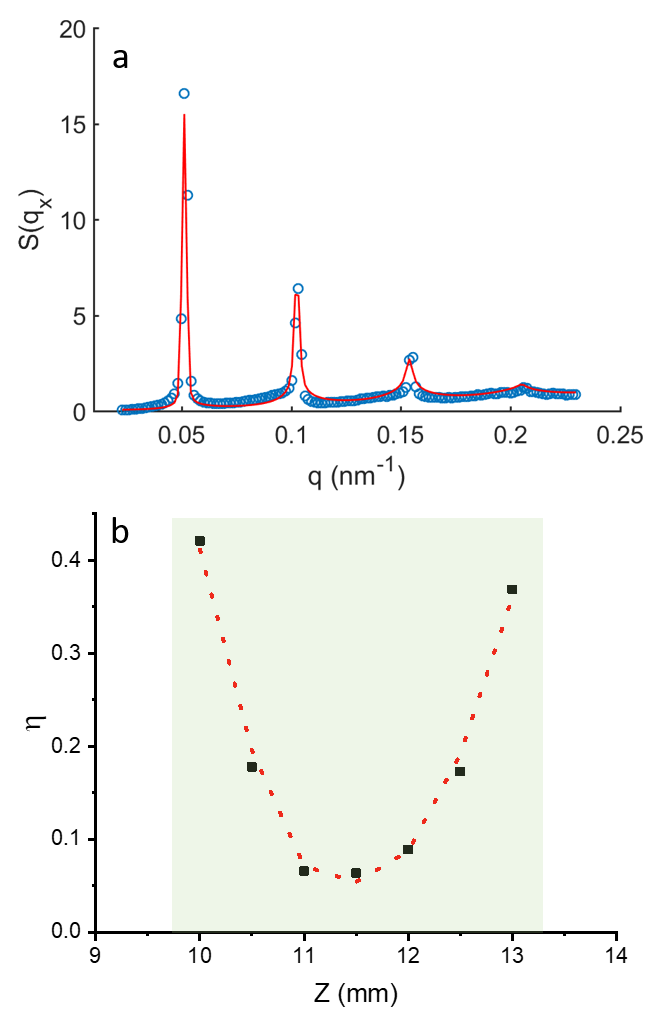
\includegraphics[width=0.5\linewidth]{callie_6.png}}
\caption{(a) Experimental structure factor along the field direction shown by red dashed line in Fig.\ref{z_scan}(c) (blue circles) along with the fit (red line) using the Nallet model described by eq.\ref{eq1:} for the smectic phase at a height $Z=11.5mm$ from the bottom of the capillary. (b) Variation of the Calli\`{e} parameter as a function of $Z$ for the smectic phase. The red dashed line is a guide to the eye but not a fit.}\label{callie}
\end{figure}

%----------------------------------------------------------------------------------------------------------------
The smectic phase is most commonly observed for amphiphilic systems where amphiphiles self-assemble in the form of bilayers, which then stack together to form a lamellar phase. We have characterized the smectic phase by borrowing the knowledge from the lamellar phase. The radially integrated structure factor $S(q_x)$ of the smectic phase can be obtained by dividing the recorded intensity, $I$, by the form factor ($\propto q_x^{-2}$). The resolution ($\Delta q$) limited $S(q_x)$ can now be described by the Nallet model~\cite{nallet1993modelling}, 
%----------------------------------------------------------------------------------------------------------------
\begin{equation}
\label{eq1:}
\begin{split}
S(q_x) = &1+2\sum_{n=1}^{N-1} (1-\frac{n}{N}) +\cos(\frac{q_x d n}{1+2\Delta q^2 d^2 \alpha(n)})\\
&\times\exp(-\frac{2q_x^2 d^2\alpha(n)+\Delta q^2 d^2 n^2}{2(1+2\Delta q^2 d^2 \alpha(n))})\frac{1}{\sqrt{1+2\Delta q^2 d^2 \alpha (n)}}
%\rho_{part}  = \frac{1}{{a_{part}b_{part^2}}} &\left[a_{core}b_{core}^2\{\rho_{sil}\phi_{pores}^{core}+\rho_{hem}(1-\phi_{pores}^{core})\} \right.\\
%& \left.+(a_{part}b_{part}^2-a_{core}b_{core}^2)\{\rho_{wtr}\phi_{pores}^{shell}+\rho_{hem}(1-\phi_{pores}^{shell})\}\right]
\end{split}
\end{equation}
%----------------------------------------------------------------------------------------------------------------
\noindent with $\alpha(n)=\frac{\eta}{4\pi^2}(\ln \pi n + \gamma)$. Here, $\gamma$ is Euler's contant and $\eta$ is the Caill\'{e} parameter, which is a measure of the fluctuations in the system; $\eta=0$ means that there are no fluctuations, while in the presence of fluctuations $\eta$ increases and the higher order Bragg peaks are smoothed out. Fig.\ref{callie}(a) shows a representative fit of the experimental data with the Nallet model, while Fig.\ref{callie}(b) represents the variation of the estimated $\eta$ as a function of $Z$. One can observe that just above the glass phase, $\eta$ is quite high with larger fluctuations in the system, followed by a sharp decrease in $\eta$ with increasing $Z$, representing a highly ordered smectic phase. However, fluctuations and hence $\eta$ again increase to higher values close to the nematic phase.\par  
%---------------------------------------------------------------------------------------------------------------- % chktex 36
Further, a careful inspection of the diffraction pattern of the nematic and smectic phases reveals an unusual but interesting feature resembling \textit{paper-clip}(Fig.~\ref{z_scan}(b,c)) shapes. This peculiar shape of the diffraction pattern is more prominent in the smectic phase, where one can clearly notice diffuse scattering lines parallel to the direction of the smectic periodicity. In the absence of the external magnetic field, particles are randomly oriented in all possible directions (fig.~\ref{Fspace_smectic}(a)). As a result, in Fourier space the structure factor is expected to be modulated in the form of spherical shells as one can see in fig.~\ref{Fspace_smectic}(b), which in turn produces a circle on the detector plane (shown by the yellow planes in fig.~\ref{Fspace_smectic}(b,c)). Since a sphere is a three dimensionally symmetrical object, it does not matter at which angle the detector plane is passing through it to get a circular/isotropic diffraction pattern (fig.~\ref{Fspace_smectic}(d)). In the presence of the external field, the particles tend to align with their short axes parallel to the field direction (fig.~\ref{Fspace_smectic}(e)). In turn, one of the rotational degrees of freedom freezes out, resulting in anisotropy in the Fourier space structure. Along the magnetic field the correlation distance is governed by the smaller particle dimension while in the orthogonal directions it is mainly dominated by their length. In the intermediate directions between these two, the gradual change of the typical correlation distance leads to this peculiar shape of the structure factor that resembles a spherocylinder (SC) as shown in fig.~\ref{Fspace_smectic}(f). % chktex 36
%In Fourier space, the structure factor becomes elongated along the direction corresponding to the short axes of the particles keeping the other two direction unchanged. As a result the structure factor is modulated in the form of a spherocylinder (SC) as shown in fig.~\ref{Fspace_smectic}(f).% chktex 12 
%----------------------------------------------------------------
\begin{figure*}[ht]
\centering{\includegraphics[width=0.95\textwidth]{Figure_Fspace_smectic_5.png}}
\caption{Schematic representation of (a) the alignment of the ellipsoids in an external field in real space. Since they align with their short axes being parallel to the field direction, they get confined in 2D planes (shown in gray) perpendicular to the direction of the field, (b) the corresponding 3D Fourier space representation of the structure factor variation in the form of a cylinder. (c) Once these layers start to get correlated, sharp Bragg spots start to appear on the axis of this cylindrical structure factor. The orange plane represents the detector plane. (d) Expected diffraction pattern on the detector plane. The sharp Bragg spots become arcs because of polycrystallinity.}\label{Fspace_smectic}
\end{figure*} 

Depending on the direction at which the detector plane intersects the Fourier space, one would therefore expect to observe either a circle, ellipse or a two dimensional projection of a SC on the detector plane. For our experimental geometry, the detector plane passes parallel to the long axis of the three dimensional spherocylinder generated in Fourier space, and one would thus expect to see a structure factor modulated in the shape shown in fig.~\ref{Fspace_smectic}(g). This expected diffraction pattern matches exactly with what we observe in the experiment for the nematic phase (fig.~\ref{Fspace_smectic}(h)). With a further increase in concentration (i.e.~moving down in the capillary) the particles get confined in 2D planes with their long axes lying on the planes (Fig.~\ref{Fspace_smectic}(i)). These planes are normal to the field direction and within each plane particle ordering is \emph{liquid}-like. Beyond a certain concentration, correlation starts to build up between these planes, resulting in a smectic phase. In an ideal smectic structure one would expect a sequence of sharp smectic reflections together with a broad intralayer scattering peak that is mostly broadened in a direction perpendicular to the layering direction. In contrast, what we observe is a paper-clip-like diffraction pattern. This peculiar shape suggests the presence of strong nematic-like fluctuations such as undulation of the smectic layers and correlations between the particles of different layers. While the correlations between the particles (that belong to different layers) along different directions lead to the horizontal diffused scattering line along the smectic periodicity, the layer undulations will lead to the appearance of the tails for higher-order Bragg peaks, which explains the multiple paper-clip-like features as highlighted in SI\@. The corresponding Fourier space structure is shown in fig.~\ref{Fspace_smectic}(j). The detector plane being parallel to the field direction and perpendicular to the x-ray beam (fig.~\ref{TEM}(c)) passes through the SC along its long axis to produce a diffraction pattern in the form of a paper-clip (fig.~\ref{Fspace_smectic}(k)) as one can observe in our experimental scattering pattern (fig.~\ref{Fspace_smectic}(l)).\par
%A closer look at the diffraction pattern of the nematic phase reveals similar diffuse scattering features arising from the formation of cylindrical structure factor (Fig.\ref{z_scan}(c)).


%----------------------------------------------------------------------------------------------------------------
\begin{figure*}[t]
\centering{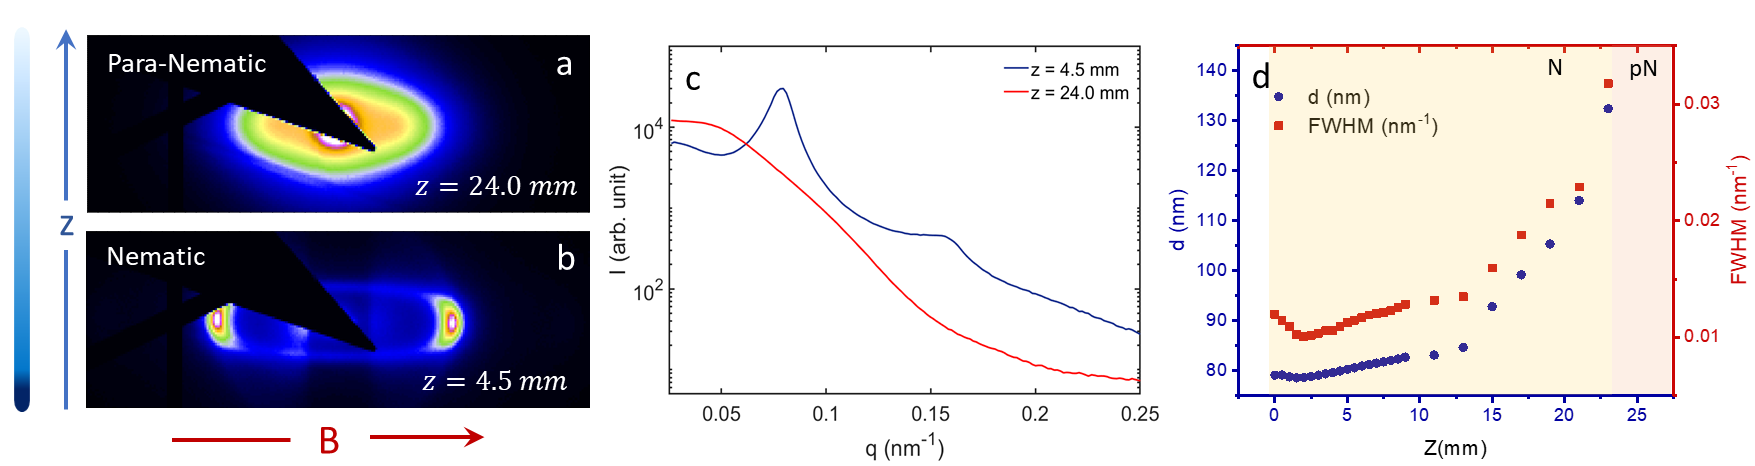
\includegraphics[width=0.95\textwidth]{z_scan_high_2.png}}
\caption{Typical 2D diffraction patterns for (a) para-nematic and (b) nematic phases at different heights of the sedimented sample for $\rho=3.69$. (c) The variation of the scattered intensity as a function of scattering vector, $q$, for the aforementioned self-assembled phases along the direction of the external field. (d) The variation of the nearest neighbor distance, $d$, and the FWHM of the nearest neighbor peaks as a function of height, $Z$ from the bottom of the capillary have been represented by the blue circles and the red squares respectively.}\label{z_scan_high}
\end{figure*}
%---------------------------------------------------------------------------------------------------------------

%----------------------------------------------------------------------------------------------------------------
\subsection{Sample $E2$ with aspect ratio $\rho_1 = 3.69$}
%----------------------------------------------------------------------------------------------------------------
In contrast to the particles with lower aspect ratio, the ones with higher aspect ratio show only two different phases in the presence of the external field. At the top of the capillaries a para-nematic phase is observed, followed by a nematic phase at the bottom (Fig.~\ref{z_scan_high}(a),(b)). In this case, the diffuse scattering due to the formation of the spherocylindrical structure factor is much more prominent in the nematic phase (Fig.~\ref{z_scan_high}(b)) itself. Fig.~\ref{z_scan_high}(c) represents the one dimensional intensity profile for the nematic and para-nematic phase along the direction of the field. The nearest neighbor distance, \emph{d}, along the direction of the field increases with $Z$ in a similar way as that of sample $E1$ (Fig.\ref{z_scan_high}(d)). In contrast, FWHM is increasing monotonically since Sample $E2$ does not show any smectic phase (Fig.~\ref{z_scan_high}(d)).   \textcolor{red}{While for our range of axial ratios the theoretical phase diagrams for ellipsoids without external fields show the same sequence of phases and only small quantitative differences in the location of the corresponding phase boundaries~\cite{radu2009solid, odriozola2012revisiting, pfleiderer2008crystal}, the existence of an external magnetic field results in dramatic changes, most notably the appearance of a hitherto unknown additional smectic phase for the smaller axial ratio. At this stage we lack any understanding of the driving forces relevant for this surprising field-induced additional phase, and we have therefore performed systematic Monte Carlo (MC) computer simulations to learn more about its origins. } \par


%----------------------------------------------------------------------------------------------------------------
\subsection{Computer Simulations}
 \textcolor{red}{Following earlier studies~\cite{martchenko2016anisotropic} of similar hematite-silica core-shell particles, we initially performed MC simulations
using a model of polydisperse hard ellipsoids (HE). Polydispersity was included through a procedure where the length $L$ and the diameter $D$ of each particle were randomly drawn from a gaussian distribution as follows:
\begin{eqnarray}
  L &=& \sigma_L\,\xi_1 + L_0\\
  D &=& \sigma_D\,\xi_2 + D_0
\end{eqnarray}
where $\xi_i$ with $i=1,2$ is a zero-mean unit-variance gaussian, $L_0=316 \nm$, $\sigma_L=26.3 \nm$, $D_0=108 \nm$ and $\sigma_D=6.98 \nm$. 
The average aspect ratio of the simulated HEs is equal to $2.9$, i.e.~close to the one of hematite-silica particles with the smaller aspect ratio investigated experimentally.  
In the following lengths will be expressed in units of $100\nm$. For both systems we simulated $N=1125$ in an orthorhombic box with periodic boundary conditions.
The external field applied to HEs induces the particles to align perpendicularly to it with a tunable strength.
Its action is implemented through the following external potential acting on each particle $i$
\begin{equation}
v_{ext}^i = k\, {( \mathbf{u}_i\cdot \hat{\mathbf{n}} )}^2
\end{equation}
where $\hat{\mathbf{n}}$ is a unit vector parallel to the field, $\mathbf{u}_i$ is a unit vector parallel to the symmetry axis of the particle,
and $k$ is parameter by which one can set the strength of the alignment. In our simulation we used $k=10^4\, k_B T$ since in the real
system the magnetic field induces a rather strong alignment of hematite-silica core-shell particles. We observe that hematite-silica core-shell particles are charged, but at high volume fractions the resulting repulsive interaction between them can be accounted for by just considering a larger effective particle volume. Hence, we expect that electrostatic repulsion between particles 
induces a shift of phase boundaries to larger packing fractions without altering qualitatively the whole phase behavior.}

\textcolor{red}{To build the equation of state (EOS) for these polydisperse HEs in the presence of the magnetic field, we performed MC simulations in the isobaric ensemble (NPT) where the three
dimensions of the orthorhombic box were allowed to change independently in order to ease the formation of mesophases. Figure~\ref{fig:sim}(a) summarizes the results obtained for the EOS of HEs. Similarly to what we have observed experimentally for hematite-silica particles with $\rho=3.72$ (Fig.~\ref{z_scan_high}) and in previous studies~\cite{martchenko2016anisotropic}, 
the polydisperse HEs with $\rho = 2.9$ exhibit two phases throughout all pressures considered in the simulations:  
a para-nematic (pN) phase (for $\phi_0\lesssim 0.45$), where the symmetry axis of the HEs is aligned perpendicularly to the 
external field $\mathbf{B}$, and a nematic phase (N) where HEs self-align also along a direction perpendicular to $\mathbf{B}$ 
({\color{green} see Sec. I of SI for more information}). It is interesting to note that the transition between these two different types of nematic phases is associated with a small variation of the volume fraction $\phi$,
thus suggesting that this transition is either weakly first order or second order.}

\textcolor{red}{Figure~\ref{fig:sim}(a) also shows a characteristic snapshot and the corresponding static structure factor at a volume fraction of $\phi \approx 0.5$. The snapshot of HEs is a prototypical example of a nematic phase, whereas no lamellar ordering is present. 
The structure factor similarly reflects the absence of any layering in the system, and it can 
be straightforwardly compared with the experimental one show in Fig.~\ref{z_scan}(b). Here we note that the structure factor that we calculated from the simulations
includes the form factor and thus represents an effective structure factor as measured by SAXS, and moreover corresponds to $\mathbf{q}$-values lying onto the plane identified by the external field (B, i.e.~y-axis) and 
a direction perpendicular to it ($z$-axis), so that a direct comparison with experiments can be made ({\color{green}see Sec.~I of SI for more details}).
Our MC simulations are thus not capable to reproduce the occurrence of a smectic phase, but instead reveal the same qualitative phase behavior as expected for HEs with larger aspect ratio, according to numerical studies reported in Ref.~\cite{martchenko2016anisotropic}. The qualitatively different phase behavior for the two aspect ratios and the existence of an additional field-induced smectic phase observed in our experiments for particles with an aspect ratio of $\rho = 2.82$ is thus not in agreement with a model of polydisperse hard ellipsoids. }



\begin{figure*}[h]
\centering{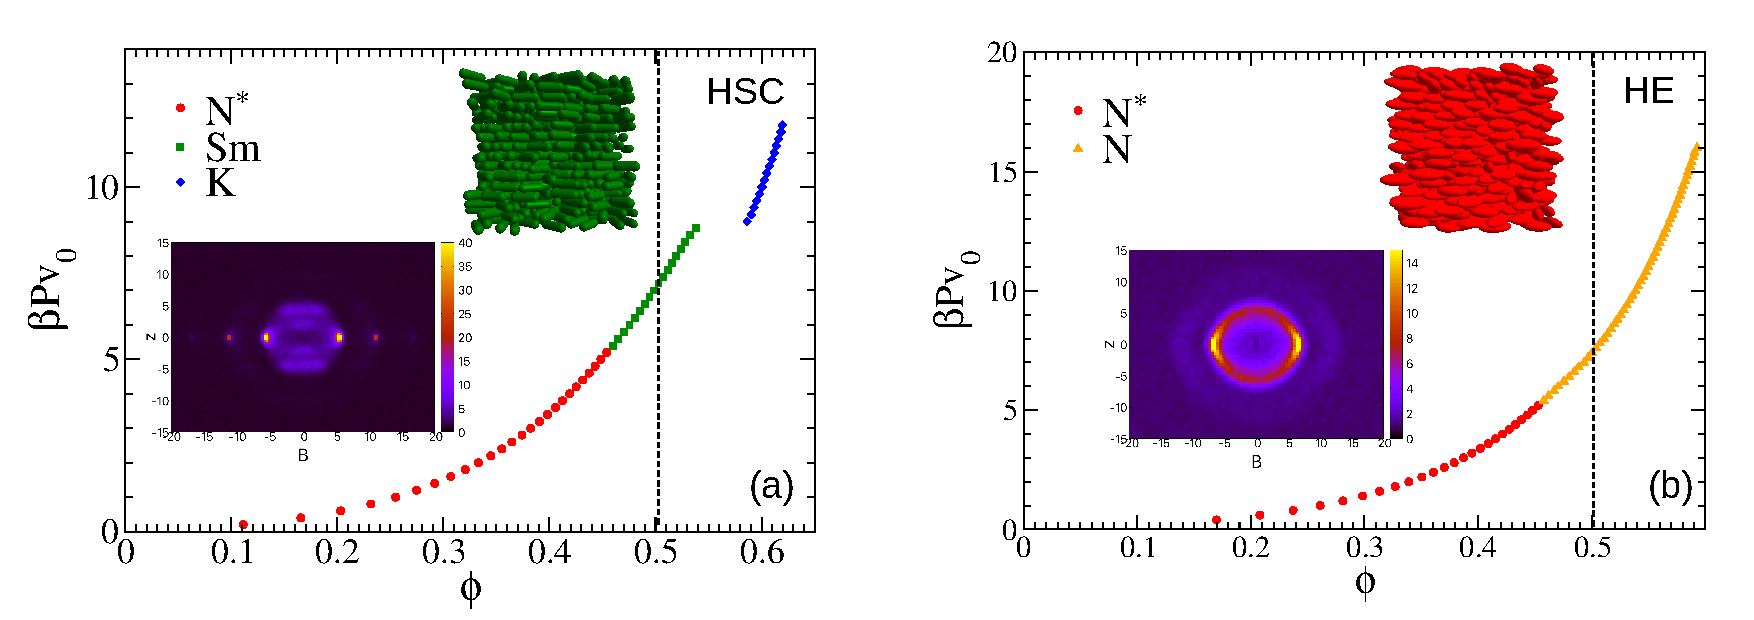
\includegraphics[width=0.95\textwidth]{mceos.pdf}}
\caption{Equation of states of (a) Hard Ellipsoids and (b) Hard Spherocylinders from Monte Carlo simulations. 
  Insets show the static structure factors and snapshots for $\phi\approx 0.50$. 
Monte Carlo Simulations}\label{fig:sim}
\end{figure*}



\textcolor{red}{A subsequent close inspection of the actual particle images using TEM (Fig.~\ref{z_scan}(a, b)) reveals
  that the two particle systems differ not only in size and aspect ratio, but that they also show subtle but systematic
  differences in their geometrical shape. Hematite-silica core-shell particles of aspect ratio $\rho=3.69$ 
  (see~\ref{z_scan}(b) and SI) closely resemble hard ellipsoids (HEs). In contrast, while the particles with the smaller
  aspect ratio $\rho=2.82$ are overall still best described by a model of an ellipsoid, they possess a    hybrid shape.
  Their midsection contains a considerably more cylinder-like (i.e.~flatter) portion that resembles a hard
  spherocylinder (HSCs),  while their ends are best described by a uni-axial hard ellipsoid model (HEs) as shown in
  Fig.\ref{z_scan}(a). These qualitative differences are further described using a more quantitative image analysis
  approach described in detail in SI.\@ In order to investigate the influence of shape more systematically, we have thus
  also performed MC simulations using a model of polydisperse hard spherocylinders (HSC), which resemble the straight
  midsections present in our particles with $\rho=2.82$ more closely ({\color{green}see Sec.~III }in the SI). Polydispersity was implemented again as
  described above for the HEs. The results from these additional simulations are summarized in Figs.~\ref{fig:sim}b,
  where we show the EOS as well as a characteristic snapshot and the corresponding static structure factor at a volume
fraction of $\phi \approx 0.5$.}

{\color{green}In the explored range of pressures,} the phase behavior of HSCs in the presence of an external field is richer 
when compared to {the one of HEs}, and we now find three phases: a para-nematic (pN) 
phase, analogous to the one observed for HEs, a smectic A phase (SmA) where the layers 
are perpendicular to the field and a uniaxial columnar crystal phase (K).
% TODO add comment on the disappearance of the SmA phase on switching off the external magnetic field
\textcolor{red}{For the HSCs we thus indeed observe the emergence of a lamellar phase for $0.45\lesssim\phi\lesssim 0.55$ 
  in agreement with the experimental results for hematite-silica particles with $\rho=2.82$ ({\color{green} see also Sec. I of SI }).
%The emergence of a SmA phase reflects what obtained from experiments for $\rho=2.82$
Interestingly, the transition from the pN to the SmA phase (as the pN-N one) 
is not associated with a significant variation of $\phi$, so that it can either
very weakly first order or second order. Differently, the transition from the SmA phase to the crystal phase
is markedly second order as expected. It is also important to point out that the SmA phase observed in the simulations is purely a field-induced effect in that
it disappears if the external field is switched off ({\color{green}see Sec. II of the SI}). }
%Concerning HSCs they also undergo a similar transition but only when the system becomes crystalline. 

\textcolor{red}{The formation of a smectic phase is further illustrated with the snapshot of HSCs shown in the inset of Figure~\ref{fig:sim}(b), where a clear lamellar ordering is apparent that is also reflected in the Bragg peaks present in the structure factor.
The distance between Bragg peaks is equal to $2\pi/d$ with $d\approx 1\,\hbox{r.u.}$, i.e.~about $D_0$, consistent with the experimental structure
factor shown in Fig.~\ref{z_scan}(c) for the smectic phase of hematite-silica particles.
Our results clearly demonstrate that the cylinder-like midsection of HSCs favors the emergence of a lamellar phase,
even if some amount of polydispersity is present in the system. }

% TODO IMPROVE THIS COMMENT 

\textcolor{red}{While the HSC simulations are capable of reproducing the occurrence of a field-induced smectic phase, a
  comparison between the experimental observations (Fig.~\ref{z_scan}) and the simulation results
  (Fig.~\ref{fig:sim}(b)) also reveals clear differences. Whereas the hematite-silica particles with $\rho_1=2.82$
  undergo a transition to a nematic N-phase, this phase is absent for HSCs, also in agreement with the phase diagram of
  monodisperse HSCs with the same aspect ratio~\cite{Bolhuis1997}. On the other hand, such a nematic phase is present
  for {\color{green}HE}, whose phase diagram mimics the one observed for the hematite-silica particles with $\rho=3.69$. This clearly
  indicates the importance of the actual shape, and of small but systematic local deviations from the ideal geometrical
  models. While these hematite-silica particles overall resemble ellipsoids, and have previously been used successfully
  in a number of studies as experimental model systems for ellipsoidal colloids, field-driven self assembly at higher
  volume fractions is obviously much more sensitive. Here the hybrid nature of the experimental particles becomes
  important, and the subtle shift from a particle that is locally better described by a spherocylinder ($\rho_1=2.82$)
  to one where the ellipsoidal geometry dominates ($ \rho=3.69$) is decisive for the resulting field-induced phase
behavior (see also Sec. III in the SI for more information on the quantitative image analysis for both particles).}



\section*{Conclusions}
%%%----------------------------------------------------------------------------------------------------------------
\textcolor{red}{In recent years we have seen considerable advances in the synthesis of complex anisotropic and often responsive colloids and their assembly into a multitude of ordered structures. In particular the use of directed self-assembly, where for example the application of external fields not only aligns the individual anisotropic building blocks and reduces their orientational degrees of freedom, but also allows one to tune the anisotropic interaction potentials between the particles, has helped to fabricate new structures~\cite{Schurtenberger2016}. This is also illustrated in this study, where we report and discuss the polymorphism exhibited by hematite-silica core-shell ellipsoidal particles undergoing field-directed self-assembly. When comparing the results obtained for two different aspect ratios, we surprisingly find not only quantitative shifts of the different phase boundaries, but discovered a novel smectic phase that has not been seen previously for prolate ellipsoidal colloids. Based on a comparison of our experimental findings with Monte Carlo computer simulations of simple anisotropic models with comparable axial ratios and polydispersity, we are led to conclude that the surprising experimental observations cannot be linked to the influence of axial ratio and external field only. Instead, {\color{green}our results} indicate the importance of subtle but systematic imperfections in the particle shape for the behavior of anisotropic particle systems in field-directed self assembly.}\par
%%%----------------------------------------------------------------------------------------------------------------
\textcolor{red}{On a more technical level, a detailed analysis of the SAXS data has provided us with an estimation of
  key structural quanities such as the orientational order parameter, $S_2$, and the fluctuation parameter, $\eta$, for
the nematic and smectic phases, respectively.} We have found that $S_2$ has very high values ($>0.8$) throughout the
whole nematic phase, indicating a highly ordered nematic phase. The ordering of the smectic phase is less at the phase
boundaries and increasing as one is moving away from the same as suggested by the variation of $\eta$. In addition, due
to the freezing of one of the rotational degrees of freedom, a new type of diffuse scattering pattern in the form of a
spherocylinder is observed. We believe that the variation of the structure factor in this particular form is a quite
general diffraction feature which can be observed for other anisotropic colloids where one out of three rotational
degrees of freedom is frozen.\par 
%%%-----------------------------------------------------------------------------------------------------------------
\textcolor{red}{Overall, our study has clearly indicated that it is not enough to consider overall shape characteristics
  (e.g., axial ratios) when attempting to understand and exploit self-assembly and field-directed self-assembly in order
  to fabricate ordered phases at high packing fractions. Experimental properties such as rotational and translational
  diffusion coefficients or structure factors of real particle dispersions such as the ones used in this study are
  indeed well described by models such as hard
  ellipsoids~\cite{martchenko2011,martchenko2016anisotropic,reufer2010morphology, reufer2012differential}. However, this
  is no longer the case when we try to understand and predict their phase behavior in field-directed self-assembly. It
  is instructive to consider the two-step synthesis process used, where the overall shape and dimensions of the
  particles are first established through the synthesis of the hematite spindle core, and the final aspect ratio is then
  selected through a coating with a silica layer of variable thickness. This appears to result not only in the expected
  variation of the axial ratio, but induces small but systematic local deviations from the overall ellipsoidal shape,
  favouring straighter {\color{green}midsections} that resemble a cylinder rather than an ellipsoid for larger shell thickness. While for
  the particles with the thinner silica shell and thus the larger aspect ratio these local shape variations are not
  sufficient to influence the phase behavior in the presence of the magnetic field, this changes dramatically for the
  thicker shell and smaller aspect ratio. Here the hybrid nature of the particle shape results in a more complex phase
  behavior that is also hybrid in nature. {\color{green}At lower volume fractions 
  a straighter midsection than the ellipsoidal one is not able to alter the phase behavior}   
  %the ellipsoid-like ends of the particles appear to
  %dominate, 
  and we observe the formation of a nematic phase that is characteristic for ellipsoids. At higher volume
  fractions however, the cylinder-like middle section now allows for the formation of a field-induced smectic phase that
  is characteristic for hard spherocylinders. These findings should not only serve as a warning when comparing
  experimental results obtained with ``real'' particles that always carry small shape imperfections with computer
  simulations using generic geometrical models, but{\color{green}, more importantly, } also as an indication that subtle variations of the resulting shape
  may lead to a much greater diversity in the accessible range of ordered phases that can be created through
field-directed self-assembly.}\par
%%%----------------------------------------------------------------------------------------------------------------
\section{Experimental Section}
%---------------------------------------------------------------------
\subsection{Synthesis and Characterization Methods}
%---------------------------------------------------------------------
Silica/hematite core/shell ellipsoidal particles of two different aspect ratios were synthesized. Hematite ellipsoids were first synthesized in water following the approach described by Ocana \emph{et al.}~\cite{ocana1999homogeneous}. They were then coated with silica layer(s) in ethanol using the method described by Graf \emph{et al.}~\cite{graf2003general}. Aspect ratio of the particles was controlled by tuning the thickness of the silica shell. Particles were purified by repeated centrifugation/redispersion cycles in water and were kept in water as a stock dispersion. Details of the synthesis and characterization of similar particles can be found elsewhere~\cite{reufer2010morphology}.\par
%---------------------------------------------------------------------
A transmission electron microscope (TEM) (TEM-CM100 microscope from Philips operating at 100 keV) was used to characterize both the size and shape of the particles. Particle size distributions were calculated by measuring at least 100 particles from TEM micrographs using the software ImageJ. For the batch of particles that we have named $E1$, we find the semi-long and semi-short axes to be $a_1 = 141\pm 16$ nm and $b_1 = 50 \pm 7$ nm respectively, leading to an aspect ratio of $\rho_1 = 2.82$, while for another batch, named $E2$, $a_2 = 133 \pm 19$ nm and $b_2 = 36 \pm 6$ nm corresponding to $\rho_2 = 3.69$. Fig.~\ref{TEM}(a) and (b) shows representative TEM images for the ellipsoids.
%---------------------------------------------------------------------
\subsection{Microradian small angle X-ray scattering}
%---------------------------------------------------------------------
For SAXS measurements, dispersions of sample $E1$ at 55wt\% and sample $E2$ at 50wt\% were placed in round capillaries with an internal diameter of 1mm (Mark tubes) that were flame sealed and stored vertically and left undisturbed for 6 months to promote particle sedimentation. Gravity induced sedimentation in the colloidal dispersions results in concentration gradients that leads to the formation of different self-assembled structures. In order to investigate the self-assembled structures, the sedimentation profiles were scanned over the full length of the capillary along the vertical directions with $Z=0$ being set at the bottom of the capillaries. SAXS measurements were performed at BM26B beam-line at ESRF, Grenoble, where a $\mu$rad-SAXS set-up which involves compound refractive lenses~\cite{petukhov2015particle} was employed. The 13 kev X-ray beam was focused on a CCD X-ray detector which was placed at a distance of 7.45 m from the sample. The data have been recorded with a PILATUS 1M detector with pixel size of 172$\times$172 $\mu$m. The detector was protected from the direct X-ray beam using a wedge-shaped beam-stop that shades the detector. The capillaries were oriented vertically with their long axis (100 mm) parallel to the gravitational field. All the measurements were carried out in presence of an external magnetic field (500 mT) which was applied after the sedimentation using a permanent magnet. The direction of the magnetic field, X-ray beam and the gravity are perpendicular to each other as shown in Fig.~\ref{TEM}(c).
%%%----------------------------------------------------------------------------------------------------------------
\section{Computational Methods}
All the results from simulations were obtained by performing up to $4\times10^7$ MC steps and by discarding the initial equilibration stage.
The initial configurations, which we used to build the EOS, were obtained by equilibrating the system at low volume fractions to have an isotropic
sample. To calculate the static structure factor we carried out NTV MC simulations starting from an initial configuration taken 
from NPT simulations for a $P$ such that $\phi\approx 0.50$. Aiming at a more direct comparison with experimental results we calculated
the static structure factors by replacing each particle (HSC or HE) with a random set of scattering points of fixed density $\rho_m$. We found
that results do not change significantly by using values of $\rho_m$ greater than about $7\times 10^{-5} \nm^{-3}$.% CARLO PLEASE CHECK THIS
Concerning the algorithms which we used for checking the overlap of HSCs and HEs, we employed the one proposed by Vega and Lago~\cite{VegaHSC1994} for HSCs and
the one proposed by Perram and Wwertheim~\cite{PerramJCP1985}. Further details on computer simulations can be found in the Supporting Information.

\section{Acknowledgments}
%%%----------------------------------------------------------------------------------------------------------------
Financial support from the European Research Council (ERC-339678-COMPASS), and the Knut and Alice Wallenberg Foundation (project grant KAW 2014.0052) is gratefully acknowledged. D. Hermida Merino is thanked for his technical support during the SAXS measurements. Crispin Hetherington is acknowledged for TEM measurement. The Nederlandse Organisatie voor Wetenschappelijk Onderzoek (NWO) is acknowledged for the provided beam-time. The Grant of Excellence Departments, MIUR-Italy (ARTICOLO 1, COMMI 314 --- 337 LEGGE 232/2016)
is gratefully acknowledged.
%%%----------------------------------------------------------------------------------------------------------------

% If in two-column mode, this environment will change to single-column format so that long equations can be displayed. 
% Use only when necessary.
%\begin{widetext}
%$$\mbox{put long equation here}$$
%\end{widetext}

% Figures should be put into the text as floats. 
% Use the graphics or graphicx packages (distributed with LaTeX2e).
% See the LaTeX Graphics Companion by Michel Goosens, Sebastian Rahtz, and Frank Mittelbach for examples. 
%
% Here is an example of the general form of a figure:
% Fill in the caption in the braces of the \caption{} command. 
% Put the label that you will use with \ref{} command in the braces of the \label{} command.
%
% \begin{figure}
% \includegraphics{}%
% \caption{\label{}}%
% \end{figure}

% Tables may be be put in the text as floats.
% Here is an example of the general form of a table:
% Fill in the caption in the braces of the \caption{} command. Put the label
% that you will use with \ref{} command in the braces of the \label{} command.
% Insert the column specifiers (l, r, c, d, etc.) in the empty braces of the
% \begin{tabular}{} command.
%
% \begin{table}
% \caption{\label{} }
% \begin{tabular}{}
% \end{tabular}
% \end{table}

% If you have acknowledgments, this puts in the proper section head.
%\begin{acknowledgments}
% Put your acknowledgments here.
%\end{acknowledgments}

% Create the reference section using BibTeX:
%%%----------------------------------------------------------------------------------------------------------------
\bibliography{ref_dubble}
\end{document}
%

% ****** End of file aiptemplate.tex ******
